\documentclass{beamer}
\usepackage{geometry}
\usepackage[english]{babel}
\usepackage[utf8]{inputenc}
\usepackage{amsmath}
\usepackage{amsfonts}
\usepackage{amssymb}
\usepackage{tikz}
\usetikzlibrary{quotes, angles}
\usepackage{graphicx}

%\usepackage{pgfplots}
%\pgfplotsset{width=10cm,compat=1.9}
%\usepackage{pgfplotstable}

\setlength{\headheight}{26pt}%doesn't seem to fix warning

\usepackage{fancyhdr}
\pagestyle{fancy}
\fancyhf{}

%\rhead{\small{2 January 2019}}
\lhead{\small{BECA / Dr. Huson / Geometry Unit 6}}

\renewcommand{\headrulewidth}{0pt}

\title{10th Grade Geometry - Unit 6: Similarity}
\subtitle{Bronx Early College Academy}
\author{Christopher J. Huson PhD}
\date{4 January 2019}

\begin{document}
\frame{\titlepage}
\section[Outline]{}
\frame{\tableofcontents}

\section{6.1 Drui: Algebra literals review. Friday 4 January}
  \frame
  {
    \frametitle{GQ: How do we solve for an unknown?}
    \framesubtitle{CCSS: HSG.CO.C.9 Prove geometric theorems \hspace{\stretch{1}} \alert{6.1 Friday 4 January}}

    \begin{block}{Do Now: Handout with algebra problems}
      \begin{enumerate}
        \item Trig applications
        \item Area and volume applications
      \end{enumerate}
    \end{block}
    Exam review. Test corrections due Monday \\
    Solving an equation for an unknown \\[0.5cm]
    Homework: Trig, area, and volume applications, handout\\
  }

\section{6.2 Drui: Dilation introduction. Monday 7 January}
  \frame
  {
    \frametitle{GQ: How do we dilate objects on the plane?}
    \framesubtitle{CCSS: HSG.CO.D.12 Congruence, geometric constructions \hspace{\stretch{1}} \alert{6.2 Monday 7 January}}

    \begin{block}{Do Now: Handout}
      \begin{enumerate}
        \item Triangle congruence, reflection handout; Perpendicular bisector construction. Orientation.
      \end{enumerate}
    \end{block}
    Test corrections due; Construction project due Friday\\
    Center of dilation and scale factor mapping pre-image$\rightarrow$image\\
    pp. 587-591\\[0.5cm] %Prep for Deltamath practice
    Homework: Dilation exercises, handout\\
  }

\section{6.2 Project: Transformations project, Monday 7 January}
  \frame
  {
    \frametitle{Construction project: Transformations}
    \framesubtitle{CCSS: HSG.CO.C.9 Prove geometric theorems \hspace{\stretch{1}} \alert{6.2}}

    \begin{block}{Three pages of transformation constructions for binder}
    \begin{enumerate}
      \item Double a line segment
      \item Construct the line of reflection
      \item Construct a dilation
    \end{enumerate}
      Grading criteria (20 points)
    \begin{enumerate}
      \item Complete and correct construction
      \item State postulate or theorem. (written steps not necessary)
      \item MLA header, center title \& last name on right
      \item Precise, elegant, mathematical aesthetic
    \end{enumerate}
    \end{block}
    Due Friday January 11
    }

\section{6.3 Drui: Deltamath. Tuesday 8 January}
  \frame
  {
    \frametitle{GQ: How do we dilate objects on the plane?}
    \framesubtitle{CCSS: HSG.CO.D.12 Congruence, geometric constructions \hspace{\stretch{1}} \alert{6.3 Tuesday 8 January}}

    \begin{block}{Do Now: Handout}
      \begin{enumerate}
        \item Construction handout
      \end{enumerate}
    \end{block}
    Deltamath assessment: dilation, reflections\\
    Deltamath homework: Algebra literals, ratios, radians (10pm deadline)
  }

\section{6.4 Drui: Dilation construction, ratios. Wednesday 9 January}
  \frame
  {
    \frametitle{GQ: How do we use scale factors to calculate dilated lengths?}
    \framesubtitle{CCSS: HSG.CO.D.12 Congruence, geometric constructions \hspace{\stretch{1}} \alert{6.4 Wednesday 9 January}}

    \begin{block}{Do Now: Handout}
      \begin{enumerate}
        \item Duplicate a segment, double a segment handout
      \end{enumerate}
    \end{block}
    Dilation construction, midline, triangle ratios\\[0.5cm]
    Homework: Take-home test, due tomorrow
  }

\section{6.5 Drui: Triangle similarity leg calcs, midline. Thursday 10 Jan}
  \frame
  {
    \frametitle{GQ: How do we define \emph{similar} objects?}
    \framesubtitle{CCSS: HSG.CO.D.12 Congruence, geometric constructions \hspace{\stretch{1}} \alert{6.5 Thursday 10 January}}

    \begin{block}{Do Now: Handout}
      \begin{enumerate}
        \item Early finishers Constructions: Dilation, line of reflection; midline
      \end{enumerate}
    \end{block}
    Right triangle dilation situations, trig\\
    Homework: Construction project due\\
  }

\section{6.6 Drui: Trig similarity. Friday 11 January}
  \frame
  {
    \frametitle{GQ: How do we understand trig ratios as similarity ratios?}
    \framesubtitle{CCSS: HSG.CO.D.12 Congruence, geometric constructions \hspace{\stretch{1}} \alert{6.6 Friday 11 January}}

    \begin{block}{Do Now: Handout}
      \begin{enumerate}
        \item Midline triangle problems handout
      \end{enumerate}
    \end{block}
    Constructions due: Dilate triangle, line of reflection; midline (spicy) \\[0.5cm]
    Similarity, triangle dilations and midline/parallels situations\\[0.5cm]
    Homework: Regents packet, complete 6 multiple choice (+3 spicy) \& 6 free response
  }

\section{6.7 Drui: Similarity ratio problems, centroid/median theorem. Monday 14 January}
  \frame
  {
    \frametitle{GQ: How do we solve similar triangles?}
    \framesubtitle{CCSS: HSG.CO.D.12 Congruence, geometric constructions \hspace{\stretch{1}} \alert{6.7 Monday 14 January}}

    \begin{block}{Do Now: Handout}
      \begin{enumerate}
        \item Regents constructions (pre-test)
      \end{enumerate}
    \end{block}
    Review take-home Regents questions\\
    Project: Regents construction packet. Due Thursday.\\
    Similarity ratio problems, centroid/median theorem\\[0.5cm]
    Homework: 6-7 Similar triangles practice
  }

\section{6.8 Drui: Deltamath. Tuesday 15 January}
  \frame
  {
    \frametitle{GQ: How do we solve for a triangle angle measure?}
    \framesubtitle{CCSS: HSG.CO.D.12 Congruence, geometric constructions \hspace{\stretch{1}} \alert{6.8 Tuesday 15 January}}

    \begin{block}{Do Now Quiz: Handout Regents constructions}
      \begin{enumerate}
        \item Preview two new Regents constructions: Aug 2017 \#28, 29\\ (early finishers \#27 and Jan 2018 \#30)
      \end{enumerate}
    \end{block}
    Deltamath assessment: Similarity, trig functions\\
    Homework: 6-8 Similar triangle ratio problems
  }

\section{6.9 Drui: Regents review. Wednesday 16 January}
  \frame
  {
    \frametitle{GQ: How do we apply the mathematics of geometry?}
    \framesubtitle{CCSS: HSG.CO.D.12 Congruence, geometric constructions \hspace{\stretch{1}} \alert{6.9 Wednesday 16 January}}

    \begin{block}{Do Now: Handout Regents constructions}
      \begin{enumerate}
        \item Preview two new Regents constructions: June 2017 \#25
      \end{enumerate}
    \end{block}
    Regents review\\[0.5cm]
    Homework: Handout
  }

\section{6.10 Drui: Regents review - Trig. Thursday 17 January}
  \frame
  {
    \frametitle{GQ: How do we apply the mathematics of geometry?}
    \framesubtitle{CCSS: HSG.CO.D.12 Congruence, geometric constructions \hspace{\stretch{1}} \alert{6.10 Thursday 17 January}}

    \begin{block}{Do Now: Handout Regents constructions}
      \begin{enumerate}
        \item Preview two new Regents constructions: June 2017 \#25
      \end{enumerate}
    \end{block}
    Regents review\\[0.5cm]
    Homework: Handout Multiple Choice Regents problems
  }

\section{6.11 Drui: Regents review. Friday 18 January}
  \frame
  {
    \frametitle{GQ: How do we apply the mathematics of geometry?}
    \framesubtitle{CCSS: HSG.CO.D.12 Congruence, geometric constructions \hspace{\stretch{1}} \alert{6.11 Friday 18 January}}

    \begin{block}{Do Now: Handout Regents constructions}
      \begin{enumerate}
        \item Transformations problems
      \end{enumerate}
    \end{block}
    Regents review\\[0.5cm]
    Homework: Study for Regents
  }


  \section{6.12 Laptops - Geogebra. Tuesday 28 January}
    \frame
    {
      \frametitle{GQ: How do we model with digital tools?}
      \framesubtitle{CCSS: HSG.CO.D.12 Congruence, geometric constructions \hspace{\stretch{1}} \alert{6.12 Tuesday 28 January}}

      \begin{block}{Do Now: Regents review and reflection}
        \begin{itemize}
          \item Results: 10 passing scores, 4 college ready
          \item Top score 75; average 53
          \item 70\% earned free response points
        \end{itemize}
      \end{block}
      GeoGebra Geometry App: www.geogebra.org/groups\\
      Enter \alert{N7BHK} for 10.1 or \alert{P9PNZ} for 10.2\\
      Set up account using your real name.\\
      Beginner Tutorials with Lesson Ideas\\
      Author: Tim Brzezinski\\[0.5cm]
      Homework: Complete Geogebra
    }

    \section{Seating Chart 10.2}
      \frame
      {
        \frametitle{Seating Chart 10.2}
        \framesubtitle{How do we work as a team?}

        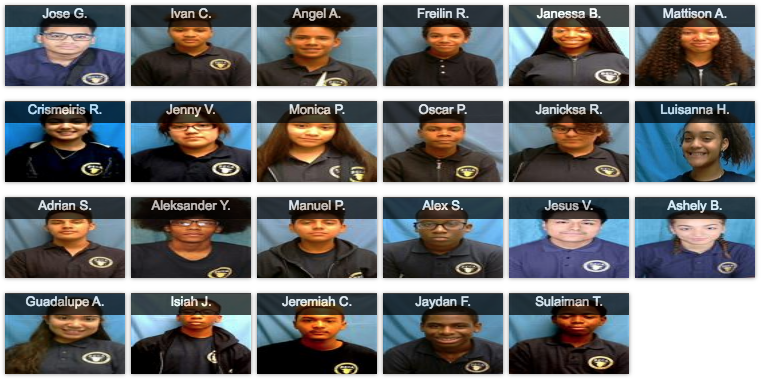
\includegraphics[width=1.05\textwidth]{seating-10B.png}

      }



\end{document}
